\section{Experimentos}
\label{sec:experiments}

O objetivo dos experimentos é validar e avaliar o sistema proposto.
Considere-se uma rede com uma topologia simples conforme mostrado abaixo: 

\begin{figure}[h!]
    \centering
    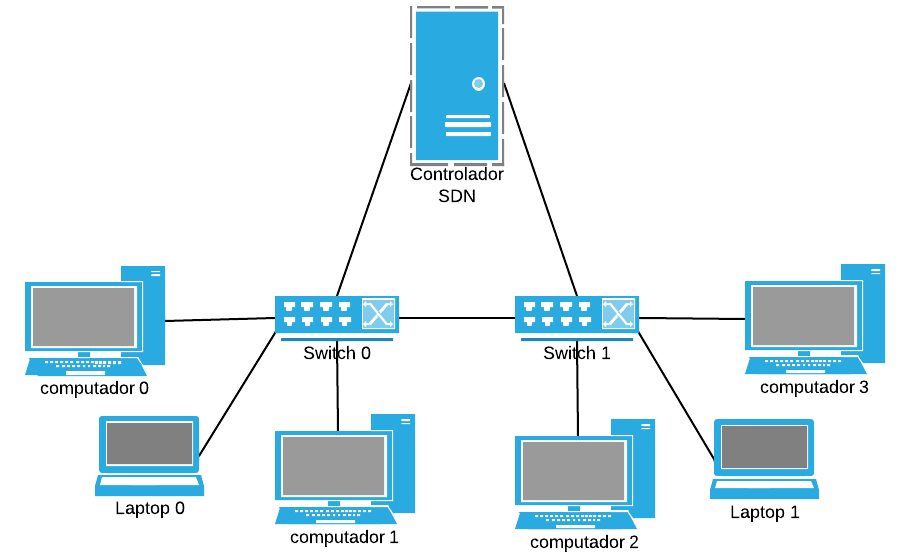
\includegraphics[scale=0.4]{mininet_topology.png}
    \caption{Topologia simples}
    \label{fig:topology}
\end{figure}

Conforme pode ser visto na figura \ref{fig:topology}, tem-se seis \emph{hosts} em sub-redes diferentes. 
Os dois \emph{switches} são controlados pela mesma instância do controlador 
POX.
Essa topologia foi configurada através do \emph{mininet} \citep{lantz2010network}. 
O mininet permite a criação de \emph{scripts} que geram topologias 
na rede simulada. 
Note que, na topologia proposta, existe um \emph{link} entre os dois 
switches.
Esse \emph{link} também é representado por uma aresta no modelo do grafo
proposto.


\subsection{Detecção de entidades}
O sistema inicia o grafo da rede vazio.
Os \emph{switches} são os primeiros a serem identificados. 
Como o controlador está ligado diretamente a eles pela interface 
\emph{OpenFlow}, um evento de \emph{ConnectionUp} é disparado 
pelo núcleo do controlador.

\begin{figure}[h!]
\centering
\begin{lstlisting}
INFO:topology.graph:SwitchJoin id: 2
INFO:topology.graph:SwitchJoin id: 1
INFO:topology.graph:1, 2
DEBUG:openflow.discovery:Dropping LLDP packet 275
INFO:topology.graph:LinkEvent fired
INFO:host_tracker:Learned 1 1 7e:e6:9b:89:39:2e got IP 10.0.0.1
INFO:topology.graph:HostJoin id: 7e:e6:9b:89:39:2e
INFO:host_tracker:Learned 2 1 62:77:44:24:13:49 got IP 10.0.0.2
INFO:topology.graph:HostJoin id: 62:77:44:24:13:49
\end{lstlisting}
\caption{Detecção de entidades}
\label{fig:detection}
\end{figure}

Nas duas primeiras linhas do \emph{log} mostrado na figura
\ref{fig:detection}, o módulo \emph{graph} foi notificado
da descoberta de dois \emph{switches} na rede.
A \emph{callback} do evento \emph{SwitchJoin} adiciona um vértice ao grafo. 
Assim, dois vértices do tipo \emph{switch} foram referenciados no grafo. 
Na linha 5, nota-se que a descoberta de um \emph{link} (entre switches).
O módulo \emph{openflow.discovery}, através do protocolo LLDP identificou 
o link entre \emph{switches}.
O grafo foi notificado e estabeleceu uma aresta entre os 
vértices (\emph{switches}).
As linhas 7 e 9 mostram a descoberta de dois hosts. 
Esses hosts foram descobertos pelo módulo \emph{host\_tracker} via 
escuta dos eventos de DHCP.
É importante ressaltar que a descoberta de \emph{hosts} também ocorre 
independente do DHCP.
Um novo pacote que passa por um \emph{switch} e não possui regra
instalada na tabela de fluxos é encaminhado ao controlador que 
dispara um evento de \emph{PacketIn}. 
Para tal, o \emph{host\_tracker} se encarrega de escutar esse evento 
e notificar o grafo através do evento \emph{HostJoin}.
O grafo, ao ser notificado, cria vértices para esses \emph{hosts} associando uma
aresta entre eles e o \emph{switch} ao qual eles estão conectados.
Dessa forma as entidades da rede são identificadas e computadas no grafo.

\subsection{Remoção de entidades}
Foram executados dois experimentos para validar a atualização do grafo
quando uma entidade (\emph{host/switch}) torna-se inativo/inalcançável.
Para o caso de remoção de \emph{host}, foi desligada a interface de 
rede de um \emph{host} via \emph{prompt} de comandos do mininet. 
O \emph{host\_tracker}, após um tempo fixo (\emph{timerInterval}) 
verifica via ARP Ping se os \emph{hosts} estão ativos.
Para esse cenário da remoção de um \emph{host}, após 30 segundos o 
\emph{host\_tracker} identificou a inatividade do \emph{host} e 
disparou o evento de \emph{HostLeave}, atualizando assim o grafo.
Para o caso do \emph{switch}, através do mininet, foi desligado um 
dos switches da topologia da figura \ref{fig:topology}.
O controlador está ligado diretamente ao \emph{switch}. 
Assim, ao ser desligado, o \emph{core} do POX dispara um evento 
de \emph{SwitchLeave} ao qual o módulo \emph{graph} está inscrito. 
Logo, o grafo é atualizado removendo o vértice do \emph{switch} e dos
\emph{hosts} ligados a ele. 

\subsection{Visualização em tempo real da rede}
Na figura \ref{fig:full_graph} é apresentado parte do grafo de uma rede
com 8 \emph{switches}, cada um com 30 \emph{hosts} conectados totalizando
248 entidades na rede.
Esse grafo é atualizado em tempo real em função dos eventos de rede ocorridos 
dentro do controlador, como entrada e saída de entidades, volume de tráfego 
na rede entre outros citados nesta seção. 

\begin{figure}[h!]
    \centering
    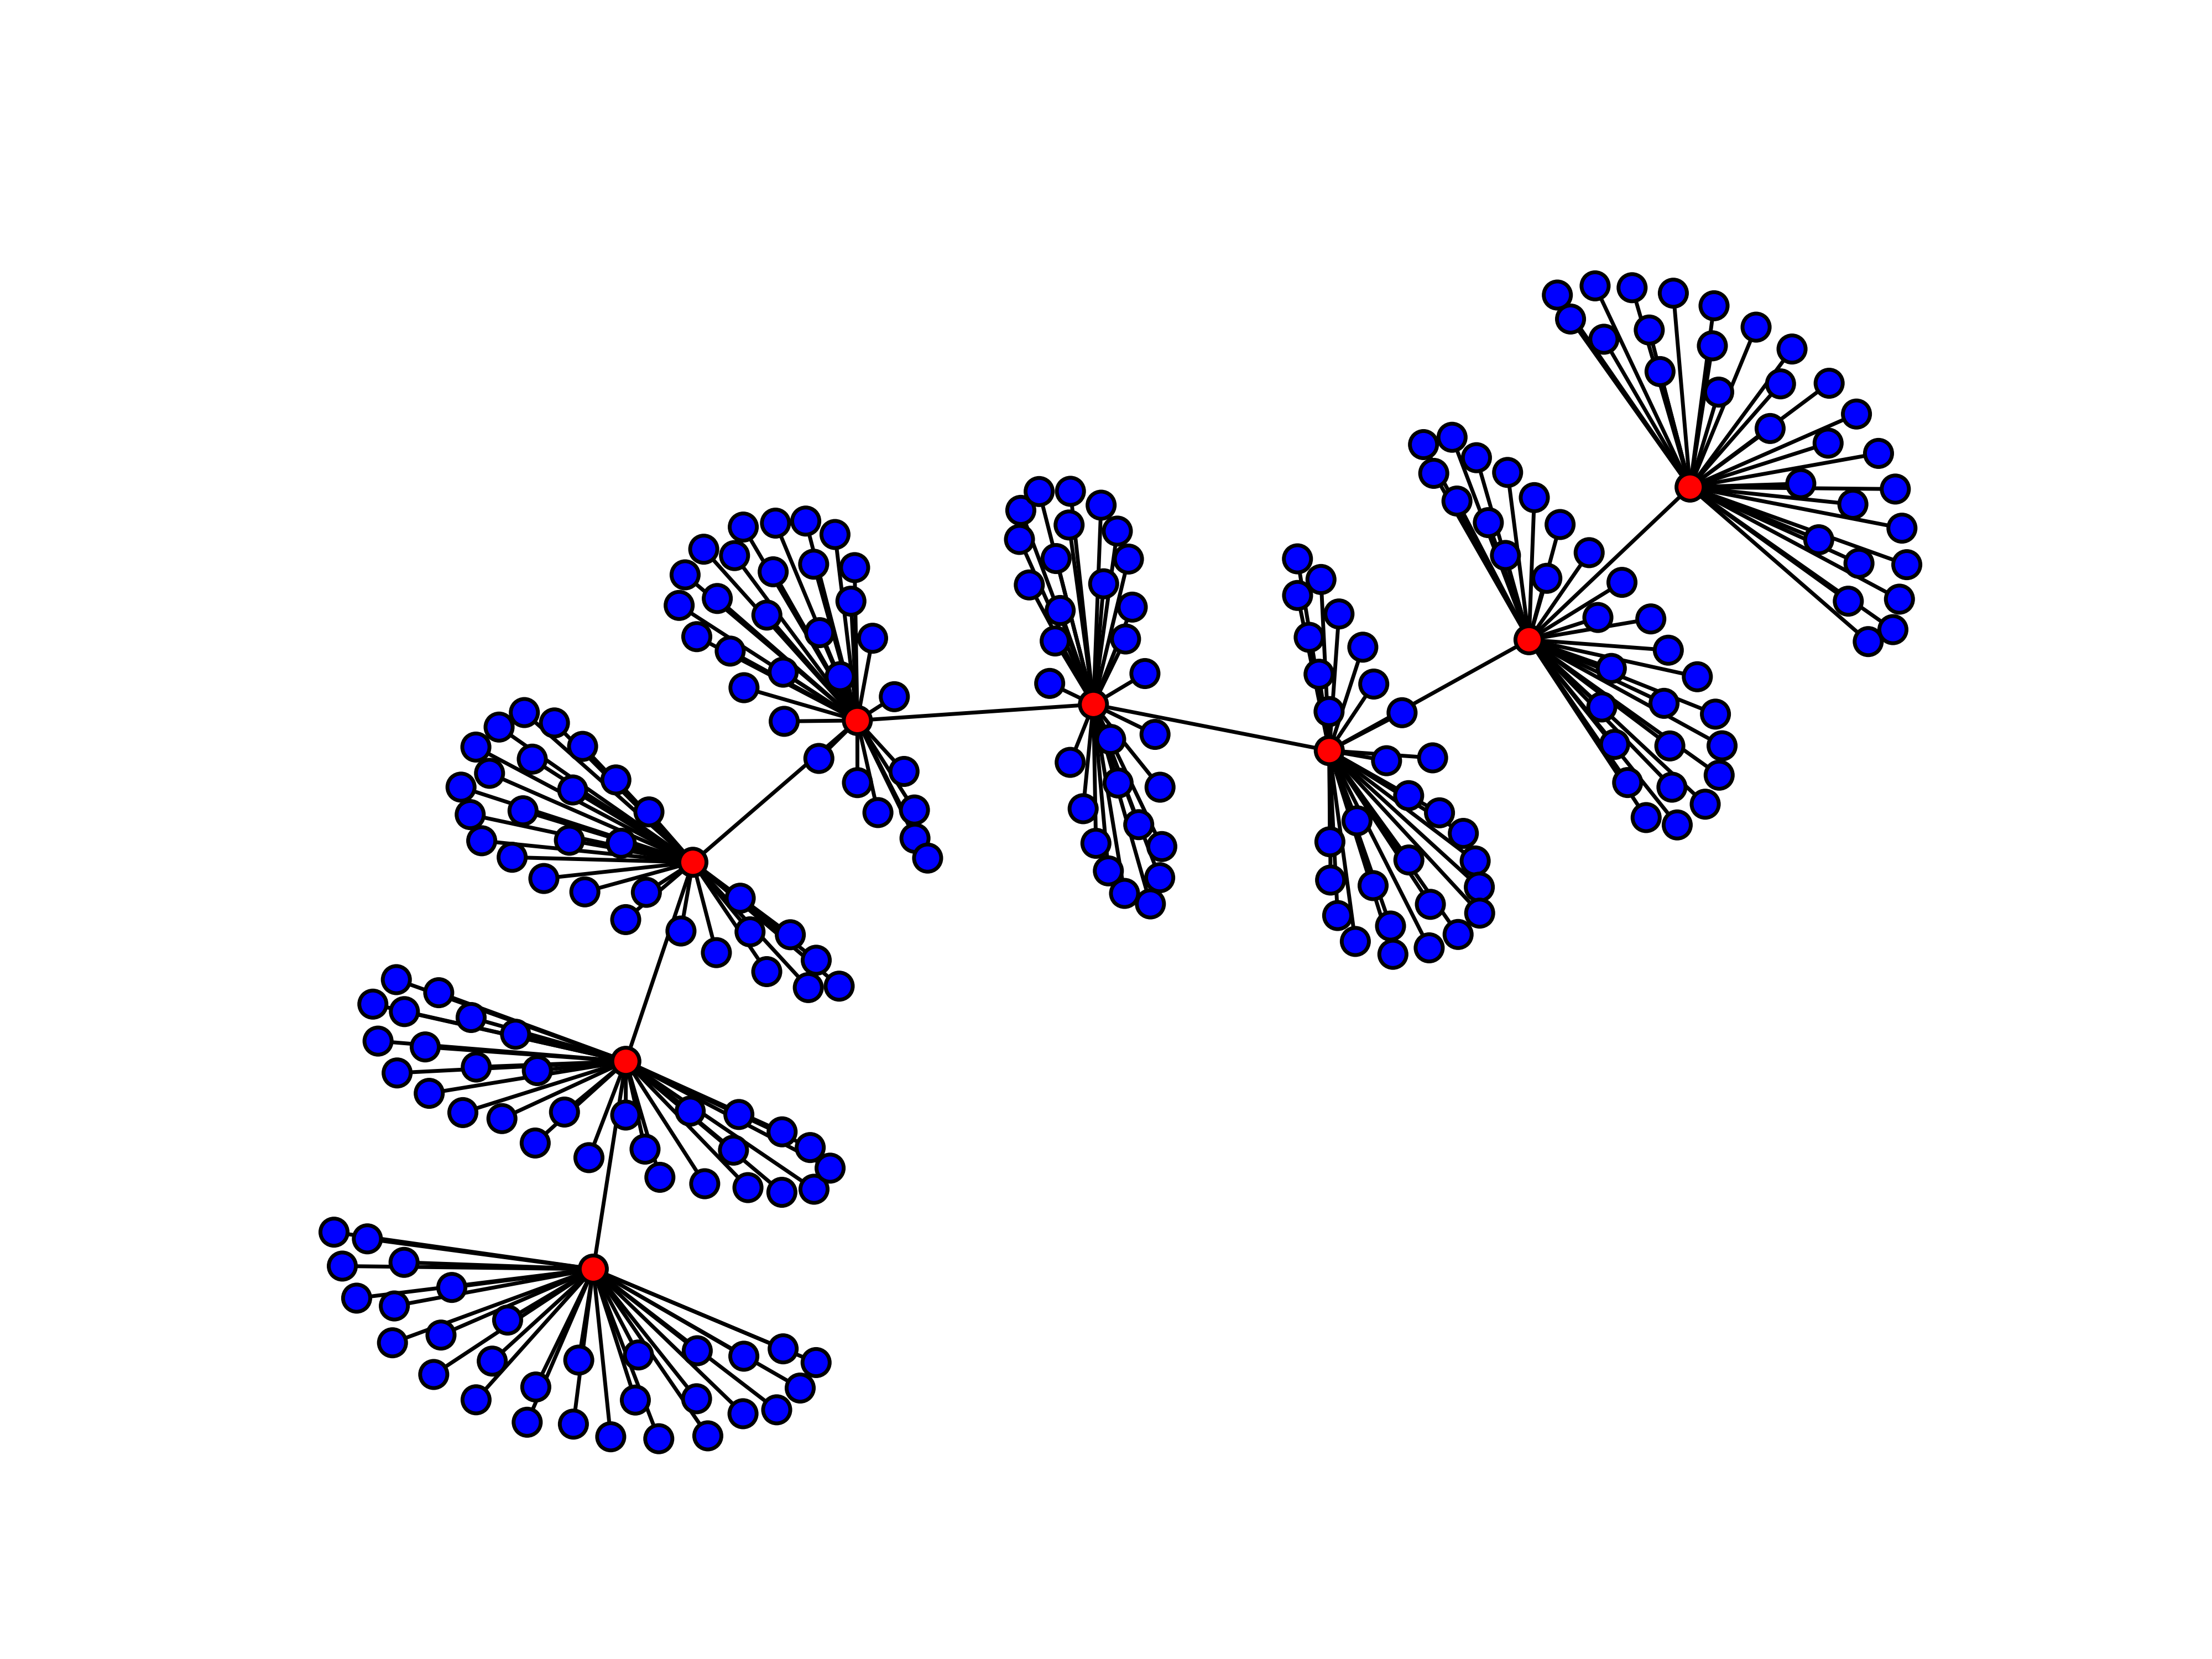
\includegraphics[scale=0.5]{full_graph.png}
    \caption{Grafo representando uma grande rede}
    \label{fig:full_graph}
\end{figure}

\subsection{Identificação de tráfego na rede}
Para computar o tráfego (TCP) na rede foi executado o programa \emph{iperf} 
como servidor no \emph{host} 'Host 0a' utilizando a topologia apresentada
na figura \ref{fig:topology}.
O \emph{host} 'Host 1e' conecta-se como cliente. 
Conformo pode ser notado na figura \ref{fig:iperf}, o tráfego 
em bytes na arestas desses \emph{hosts} é superior ao demais \emph{hosts}.
No momento em que foram lidos os contadores \emph{OpenFlow} e computados
os pesos das arestas, obteve-se um tráfego de 55894 bytes através do caminho
entre os dois \emph{hosts} citados.
Os valores apresentados para os demais \emph{hosts} (41 bytes) são referentes
ao tráfego ARP PING disseminado pelo módulo \emph{host\_tracker}
O experimento com o \emph{iperf} mostrou uma taxa de envio 
(\emph{throughput}) entre os \emph{hosts} de 300 Mega bits por segundo.

\begin{figure}[h!]
    \centering
    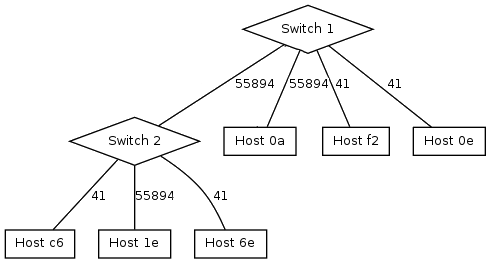
\includegraphics[scale=0.8]{graph_iperf.png}
    \caption{Tráfego TCP (em bytes) entre os hosts ’Host 1e’ e ’Host 0a’}
    \label{fig:iperf}
\end{figure}

\subsection{Árvore Geradora Mínima}
Uma árvore geradora mínima é mantida em tempo real sobre o grafo
da rede. 
Quando o grafo adiciona, remove ou atualiza arestas/vértices a árvore 
geradora mínima é computada. 
Outros módulos podem utilizá-la através da API do módulo em grafos.

Árvores geradoras mínimas são essenciais em diversas tarefas no gerenciamento
de redes.
Tarefas como disparar 'alarmes' quando a árvore estiver desconexa ou 
contenha \emph{loops}, conforme mostrado em \citep{schmid2013exploiting}.
É possível imaginar um sistema distribuído que consulte a árvore geradora
mínima para executar um algoritmo de propagação de mensagem \emph{flood} 
de maneira inteligente e menos custosa para 
a rede \citep{Monsanto:2013:CSN:2482626.2482629}.
Uma rede com múltiplos \emph{switches} pode implementar um 
balanceamento de carga eficiente que considere o tráfego nas arestas
utilizando a árvore geradora mínima em tempo real.
Além disso, é possível imaginar soluções como o \emph{Green MST}, 
apresentado em \citep{prete2012energy}. 
Uma abordagem em SDN utilizando uma árvore geradora mínima 
para reduzir o consumo elétrico da rede utilizando métricas da 
camada de aplicação. 
